\newpage
\section{Chachowski Jakub}
\raggedright
wzór: $\sqrt{\Delta} = \sqrt{b^2-4ac}$


\begin{figure}[htbp!]
\begin{center}
    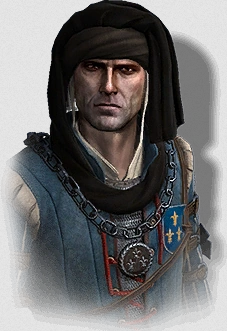
\includegraphics{pictures/kupiec.png}
    \caption{Emhyr var Emreis — kupiec korzenny}
    \label{fig:emhyr}
\end{center}
\end{figure}


\begin{figure}[htbp!]
    \begin{table}[htbp!]
\begin{center}

    \begin{tabular}{|cc|c|c|c|c|c|c|}
        \hline
        \multicolumn{2}{c}{AWG}  &  \multicolumn{2}{c}{Średnica}  &  \multicolumn{2}{c}{Przekrój}  & \multicolumn{2}{c}{Rezystancja} \\
        \hline
         && cm & in & $mm^2$ & kcmil & $\Omega/km$ & $\Omega/tysiąc stóp$ \\
        \hline
        1 && 7,348 & 0,2893 & 42,4 & 83,7 & 0,4066 & 0,1239 \\
        \hline
        2 && 6,544 & 0,2576 & 33,6 & 66,4 & 0,5127 & 0,1563\\
        \hline
        4 && 5,189 & 0,2043 & 21,2 & 41,7 & 0,8152 & 0,2485\\
        \hline
        6 && 4,115 & 0,1620 & 13,3 & 26,3 & 1,296 & 0,3951\\
        \hline
        8 && 3,264 & 0,1285 & 8,37 & 16,5 & 2,061 & 0,6282\\
        \hline
        10 && 2,588 & 0,1019 & 5,26 & 10,4 & 3,277 & 0,9989\\
        \hline
        12 && 2,053 & 0,0808 & 3,31 & 6,53 & 5,211 & 1,588\\
        \hline
        16 && 1,291 & 0,0508 & 1,31 & 2,58 & 13,17 & 4,016\\
        \hline
    \end{tabular}
    \caption{AWG}
\end{center}  
\end{table}
\end{figure}

lista punktowana:
\begin{itemize}
    \item test
    \item test2
    \item text3
\end{itemize}

lista numerowana:
\begin{enumerate}
    \item test
    \item test2
    \item text3
\end{enumerate}


\paragraph{}
Lorem ipsum dolor sit amet, consectetur adipiscing elit. Phasellus id sapien facilisis, tempus leo vel, malesuada ante. Nunc tristique id ipsum id iaculis. Aenean ultricies sodales nibh. Nullam malesuada, purus congue ullamcorper convallis, magna felis sodales turpis, ultrices pharetra tortor justo eget odio. Nunc ante turpis, feugiat ut ornare feugiat, laoreet ut dui. Fusce a arcu dui. Morbi sit amet lacinia arcu. Pellentesque eu libero sapien. Aliquam dictum ligula non semper lacinia. Integer commodo ante eu lacus sagittis scelerisque. Vestibulum ante ipsum primis in faucibus orci luctus et ultrices posuere cubilia curae; Aenean mattis massa a turpis suscipit interdum.
\paragraph{}
Litwo! Ojczyzno moja! ty jesteś jak zdrowie. Ile cię trzeba cenić, ten tylko się dowie, Kto cię stracił. Dziś piękność twą w całej ozdobie Widzę i opisuję, bo tęsknię po tobie.Panno Święta, co Jasnej bronisz Częstochowy I w Ostrej świecisz Bramie! Ty, co gród zamkowy Nowogródzki ochraniasz z jego wiernym ludem!Jak mnie dziecko do zdrowia powróciłaś cudem (Gdy od płaczącej matki pod Twoję opiekę Ofiarowany, martwą podniosłem powiekę I zaraz mogłem pieszo do Twych świątyń progu Iść za wrócone życie podziękować Bogu), Tak nas powrócisz cudem na Ojczyzny łono.Tymczasem przenoś moję duszę utęsknioną Do tych pagórków leśnych, do tych łąk zielonych, Szeroko nad błękitnym Niemnem rozciągnionych Do tych pól malowanych zbożem rozmaitem, Wyzłacanych pszenicą, posrebrzanych żytem; Gdzie bursztynowy świerzop, gryka jak śnieg biała, Gdzie panieńskim rumieńcem dzięcielina pała, A wszystko przepasane, jakby wstęgą, miedzą Zieloną, na niej z rzadka ciche grusze siedzą.
\paragraph{}
Pewien kupiec został ukazany na zdjęciu nr \ref{fig:emhyr} na stronie nr \pageref{fig:emhyr}
